\documentclass{note}
\usepackage{mypackage}

\renewcommand{\thefootnote}{\fnsymbol{footnote}}

\title{计算机网络笔记}
\author{陈鸿峥}
\date{{\builddatemonth\today}\protect\footnote{\text{Build \builddate\today}}} % protect!

\begin{document}

\maketitle
\renewcommand{\thefootnote}{\arabic{footnote}}
\setcounter{footnote}{0}

\setcounter{tocdepth}{2}%设置深度
\tableofcontents

\bigskip\bigskip
本课程使用的教材为James F.~Kurose和Keith W.~Ross的《计算机网络---自顶向下方法(第七版)》。

% !TEX root = main.tex

\section{计算机系统概述}
\subsection{计算模型}
\begin{itemize}
	\item 图灵机(1936)
	\item 冯诺依曼体系结构(1945)\footnote{非冯诺依曼体系结构:并行计算、量子计算、生物计算} --- 存储程序原理(\textbf{运算器}为中心)\\
	计算机采用\textbf{二进制}表示机器指令和数据,按照程序指令\textbf{顺序}执行
\begin{center}
\begin{tikzcd}
& & \text{存储器}\arrow{d} & & \\
\quad\arrow{r} & \text{输入设备}\arrow{r} & \text{运算器}\arrow{r}\arrow{d}\arrow{u} & \text{输出设备}\arrow{r} & \quad\\
& & \text{控制器}\arrow{u}\arrow{lu}\arrow{ru}\arrow[bend left]{uu} & &
\end{tikzcd}
\end{center}
而现在由于计算不是瓶颈,存储访问成为了瓶颈,故现代微机以\textbf{存储器}为中心
\begin{center}
\begin{tikzcd}
& & \text{运算器}\arrow{d} & & \\
\quad\arrow{r} & \text{输入设备}\arrow{r} & \text{存储器}\arrow{r}\arrow{d}\arrow{u} & \text{输出设备}\arrow{r} & \quad\\
& & \text{控制器}\arrow{u}\arrow{lu}\arrow{ru}\arrow[bend left]{uu} & &
\end{tikzcd}
\end{center}
\end{itemize}
[运算器、控制器](CPU)、存储器为计算机的核心,合称主机;外围设备,简称外设,指除主机外的其他设备,包括IO设备、外存等

计算机中的信息仍用二进制表示的原因:由物理器件性能决定
\begin{itemize}
	\item 二进制只有两种状态,容易找到具有2个稳定状态并且状态转换容易控制的物理器件(数字电路)
	\item 二进制编码运算规则简单
	\item 二进制的0、1与二值逻辑一致,容易实现逻辑运算
\end{itemize}
% There are two reasons computers use the binary system:
% 1.Two clearly distinct states that provide a safety range for reliability.
% 2.Least amount of necessary circuitry, which results in the least amount of space, energy consumption, and cost.

\subsection{计算机的发展历程}
按发展历程可分为:电子管、晶体管、集成电路、(超)大规模集成电路四代计算机
\par重大历史事件如下
\begin{center}
\begin{tabular}{|c|c|c|c|}
\hline
% 年份 & 姓名 & 事件 & 备注 \\
1904 & 弗莱明(Fleming) & 二极管 & \\\hline
1907 & 德福雷斯特(De Forest) & 三极管 & \\\hline
1938 & 香农(Shannon) & 布尔代数与二值电子器件(继电器) & 奠定数字电路基石 \\\hline
1946 & & 第一台通用计算机ENIAC & 十进制 \\\hline
1947 & \begin{tabular}{c}布莱顿(Brattain)\\
巴丁(Bardeen)\end{tabular} & 点接触晶体管 & \\\hline
1949 & 肖克利(Shockley) & 结型晶体管(1949) & 1956诺贝尔奖\\\hline
1950 & & 二进制和存储程序EDVAC & 实现冯诺依曼设想(组合进步) \\\hline
1958 & Jack Kilby & 集成电路 & 2000诺贝尔奖 \\\hline
1965 & Moore & 摩尔定律 & \begin{tabular}{c}
在价格不变的情况下,每18个月芯片上\\
晶体管数目翻倍,性能也提升一倍
\end{tabular}\\\hline
1971 & Intel & 第一款微处理器4004 & 10$\mu$m\\\hline
\end{tabular}
\end{center}

\subsubsection{单处理器(1971-2002)}
性能提升主要手段
\begin{itemize}
	\item 提升工作主频:KHz增长至GHz(生产工艺进步,流水线级数增加)
	\item 指令级并行(ILP)
\end{itemize}
\begin{proposition}[安迪-比尔定律]
Andy gives, Bill takes away. 安迪是原Intel CEO,比尔是原微软CEO,硬件厂商靠软件开发商用光自己提供的硬件资源得以生存
\end{proposition}
但遇到频率墙和功耗墙
\[\text{功耗(power)}\propto 1/2\times\text{CMOS电容}\times\text{电压}^2\times\text{转换(01)频率}\]
\par
2004年,Intel放弃4GHz Pentium4芯片开发,因无法解决散热问题,通过加快主频提升处理器性能的路走到尽头

\subsubsection{多核处理器(2005-)}
采用多核处理器不过是将硬件的问题丢到软件\footnote{“向多核的转变并不是因为我们在软件或体系结构技术上取得了中大突破而带来的。相反,这种转变是当单处理器体系结构发展遇到了难以克服的巨大障碍时,我们被迫作出的一种选择。”---Kurt Keutzer (UCB), \emph{The Landscape of Parallel Computing Research: A View from Berkeley}}
\begin{theorem}[阿姆达尔(Amdahl)定律]
\label{thm:amdahl}
\[\text{改进后的执行时间}=\text{受改进影响部分的执行时间}/\text{改进提高的倍数}+\text{不受影响的执行时间}\]
\[S_A=\frac{1}{s+(1-s)/N},\]
\end{theorem}
对计算机系统的某个部分采用并行优化措施后所获得的计算机性能的提高是有上限的,上限由串行部分所占的比例决定
\begin{theorem}[古斯塔夫森(Gustafson)定律]
\[S_G=(s'+p'\times N)/(s'+p')=N+(1-N)\times s',\]
其中,$s'$和$p'$为程序串行部分与可并行化部分在并行系统上执行的时间占总时间的比例,$N$为处理器数量,简便起见设总时间$s'+p'=1$
\end{theorem}
打破Amdahl定律\textbf{问题规模不变}的假设,任何足够大的任务都可以被有效地并行化,只要问题规模可扩展,并行所带来的加速比就可以扩展


\subsection{计算机系统的层次结构}
\begin{center}
\begin{tikzcd}
\text{高级语言层}\arrow{d}{}\\
\text{汇编语言层}\arrow{d}{}\\
\text{操作系统层}\arrow{d}{}\\
\text{指令系统层}\arrow{d}{}\\
\text{微体系结构层}\arrow{d}{}\\
\text{数字逻辑层}
\end{tikzcd}
\end{center}
程序编译运行过程:
\begin{center}
\begin{tikzcd}
\text{高级语言}\quad\arrow{r}{\text{预编译、编译}} & \quad\text{汇编语言}\arrow{r}{\text{汇编}} & \text{目标文件(二进制)}\arrow{r}{\text{链接}} & \text{可执行文件(二进制)}\arrow{d}{\text{加载}}\\
& & \text{电路上的电信号}\quad & \quad\text{二进制机器指令流(硬盘$\to$存储器)}\arrow[swap]{l}{\text{CPU取指译码}}
\end{tikzcd}
\end{center}
计算机内部工作过程:逐条执行加载到内存中的二进制机器指令流的过程

指令执行分为两个阶段,周期性重复性进行:
\begin{itemize}
	\item 取指阶段:CPU从内存中读取指令,程序计数器(PC)保存要被要被取出的\textbf{下一条}指令的地址,除非遇跳转指令,否则都加一个增量\footnote{程序计数器(Program Counter)是一个实际存在的寄存器吗? - Belleve的回答 - 知乎 \url{https://www.zhihu.com/question/22609253/answer/21965180} PC每次增加\textbf{一条指令的长度/寻址粒度},在MIPS中一条指令长4字节,寻址粒度1字节,故每次PC加4;而x86体系指令长度不定,每次增加量会变化}
	\item 执行阶段:对取出的指令译码后执行
\end{itemize}
软件系统可分为系统软件和应用软件

\subsection{计算机结构的八个想法}
\begin{enumerate}
	\item 摩尔(Moore)定律:集成电路资源每$18-24$个月翻倍
	\item 抽象(abstraction):简化设计
	\item 加速常用操作(Make common case fast):见定理\ref{thm:amdahl}
	\item 并行(parallelism)
	\item 流水线(pipelining)
	\item 预测(prediction)
	\item 内存等级制(hierarchy)
	\item 冗余实现可靠性(redundancy):检测故障及解决
\end{enumerate}

\subsection{基本指标}
表示计算机通信带宽时
\begin{center}
\begin{tabular}{ccccccc}\hline
KB(yte) & MB & GB & TB & PB & EB & ZB\\\hline
$10^3$ & $10^6$ & $10^9$ & $10^{12}$ & $10^{15}$ & $10^{18}$ & $10^{21}$\\\hline
\end{tabular}
\end{center}
表示计算机存储二进制时
\begin{center}
\begin{tabular}{ccccccc}\hline
KiB(yte) & MiB & GiB & TiB\\\hline
$2^{10}$ & $2^{20}$ & $2^{30}$ & $2^{40}$\\\hline
\end{tabular}
\end{center}
\begin{itemize}
	\item 位(bit/b):计算机处理、存储、传输信息的最小单位
	\item 字节(Byte/B) $1\text{ Byte}=8\text{ bit}$:现代计算机主存按字节编制,字节是最小可寻址单位
	\item 字(Word):表示被处理信息的单位,用来度量数据类型的宽度\footnote{字长是指CPU中\textbf{数据通路的宽度},等于CPU内部总线的宽度或运算器的位数或通用寄存器的宽度;字和字长的宽度可以一样,也可以不同,通常是字节的整数倍}
\end{itemize}
\par 一台32位的电脑,一个字等于4个字节,字长为32位;若字长为16位,则一个字等于2字节.
\par 4字节相当于8位16进制编码

\subsection{性能评价}
\label{subsec:performance}
CPU主频:对同一型号计算机,主频越高,完成指令一个执行步骤时间越短
\[\text{计算机的性能(Performance)}=1/\text{执行时间(Execution time)}\]
按照单位(量纲)进行换算即可
\[\begin{aligned}
\text{CPU执行时间(s)}&=\text{执行程序所需CPU时钟周期(cyc)}\times\text{时钟周期s/cyc)}\\
&=\text{指令数目(ins)}\times\text{CPI(cyc/ins)}\times\text{时钟周期(s/cyc)}
\end{aligned}\]
程序性能对执行事件的影响:
\begin{center}
\begin{tabular}{|c|c|c|c|}\hline
 & 指令数 & CPI & 时钟周期\\\hline
算法、编程语言、编译器 & $\times$ & $\times$ & \\\hline
指令集 & $\times$ & $\times$ & $\times$ \\\hline
计算机组成 & & $\times$ & $\times$ \\\hline
实现技术 & & & $\times$\\\hline
\end{tabular}
\end{center}
体系结构=指令集体系结构(功能定义与设计)+计算机组成(考虑用什么材料)\\
举例来说:
\begin{itemize}
	\item 指令集(ISA)考虑:是否提供乘法指令
	\item 组成(Organization)考虑:如何实现乘法指令(专门乘法器还是加法器+移位器)
	\item 实现技术(Technology)考虑:如何布线、用什么材料和工艺
\end{itemize}

% 带有处理器的设备一般称为智能化设备
% 完整的计算机系统应包括配套的硬件设备和软件系统
% !TEX root = main.tex

\section{物理层}
在\textemph{直连网}中传输原始比特流,不管包。
需要做的事情:
\[\text{信息源}\to\text{调制/编码}\to\text{信道传输}\to\text{解调/解码}\to\text{目的地}\]
其中调制解调为模拟信号,编码解码为数字信号。

信息能够被解释为数据(data),用符号(sign)记录,用信号(signal)(光、电)传递(transmit),\\用熵(entropy)测量。
\begin{itemize}
	\item 模拟信号-传输:连续取值(连续波长而不是连续信息),放大器(amplifier)
	\item 数字信号/跳变信号-传输:离散取值,中继器(repeater)
\end{itemize}

\subsection{编码方式}
\subsubsection{模拟信号}
载波信号(carrier)一般采用正弦波信号:角频率$\omega$、频率$f$、周期$T$、振幅$A$、相位$\varphi$
\begin{itemize}
	\item 频移键控(frequency-shift keying, FSK):通过不同频率表示不同信息0/1
	\item 幅移键控(amplitude-shift keying, ASK):通过不同振幅表示不同信息
	\item 相移键控(phase-shift keying, PSK):通过不同相位表示不同信息
	\item 正交调幅(quadrature amplitude modulation, QAM):用不同的\textemph{振幅和相位的组合}表示不同的多位信息,如$000\thicksim 111$
\end{itemize}

\subsubsection{数字信号}
\begin{enumerate}
\item 单极编码(unipolar):0V即0,$+E$V为1,但是会产生两种漂移
\begin{itemize}
	\item 时钟漂移:发送方和接收方采用\textemph{不同的时钟信号},或长时间没有校正信号;一定要\textemph{有跳变}
	\item 基线漂移:线很长会有,长时间传输\textemph{相同电平信号}导致积累很多\textemph{同种电荷},最后导致信号整体偏离基准线;一定要\textemph{有变化/正负}
\end{itemize}
\item 不归零编码/双极编码(non-return-to-zero/bipolar, NRZ) :$-E$为0,$+E$为1,解决基线漂移问题(平衡01);全是0或全是1,还是没法区分
\item 不归零反转编码(Inverted, NRZI):\textemph{差分}码波形,相邻码元的电位改变表示1,而电位不改变表示0;也可以反过来。 该表示方法与码元本身电位或极性无关,而仅与相邻码元的电位变化有关
\item 曼彻斯特(Manchester)编码:从相邻时刻的中间起降$-E\thicksim +E$,$0\to 10, 1\to 01$,\textemph{可克服时钟漂移和基线漂移};频率高,传输有问题,对传输介质要求高
\item 差分曼彻斯特编码:在每一位开始时间如果跳变(当前编码与原数据不同)则为0,否则为1,且\textemph{中间也要跳变}
\begin{figure}[H]
	\centering
	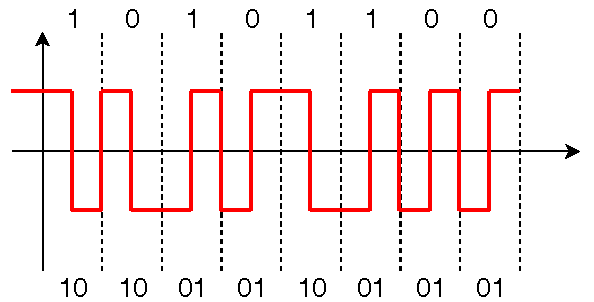
\includegraphics[width=0.5\linewidth]{fig/network-manchester.pdf}
\end{figure}
\item 4B/5B编码:用5比特代表4比特,多一位冗余;每个编码没有多于1个前导零和多于2个末端零,即\textemph{最多3个0};
防止跳变过多,又可消除基线漂移和时钟漂移
\begin{center}
\begin{tabular}{|c|c||c|c|}\hline
4B & 5B & 4B & 5B\\\hline\hline
0000 & 11110 & 1000 & 10010\\\hline
0001 & 01001 & 1001 & 10011\\\hline
0010 & 10100 & 1010 & 10110\\\hline
0011 & 10101 & 1011 & 10111\\\hline
0100 & 01010 & 1100 & 11010\\\hline
0101 & 01011 & 1101 & 11011\\\hline
0110 & 01110 & 1110 & 11100\\\hline
0111 & 01111 & 1111 & 11101\\\hline
\end{tabular}
\end{center}
\end{enumerate}

\subsection{物理介质}
\subsubsection{分类}
\begin{enumerate}
\item 有线介质
\begin{itemize}
	\item 双绞线:
	\begin{itemize}
		\item 非屏蔽双绞线(unshielded twisted pair, UTP):四对线(绿绿白、橙橙白、蓝蓝白、棕棕白),cat5/cat5e百兆以太网,cat6千兆以太网\footnote{1KB(Kilobyte,千字节),1MB(Megabyte,兆字节,简称``兆''),1GB(Gigabyte,吉字节,又称``千兆'')}
		\item 屏蔽双绞线(STP)
	\end{itemize}
	\item 同轴电缆(coaxial cable)
	\item 光导纤维(optical fiber):利用光的全反射性质
	\begin{itemize}
		\item 单模光纤(single mode):最大传输速率
		\item 多模光纤:阶跃(step-index)光纤、渐变(graded-index)光纤
	\end{itemize}
\end{itemize}
\item 无线介质:地面微波、WiFi、3G网络、卫星
\end{enumerate}

\subsubsection{多路复用方式}
\begin{itemize}
	\item 时分多路复用(time division multiplexing, TDM):时间域被分成周期循环的一些小段,每段时间长度是\textemph{相同}的,每个时段用来传输一个子信道
	\item 频分多路复用(frequency, FDM):\textemph{无线电台}常用
	\item 波分多路复用(wavelength, WDM):利用多个激光器在单条光纤上同时发送多束\textemph{不同波长}激光的技术
	\item 码分多路复用(code, CDM):利用各路信号码型结构正交性而实现多路复用
	\item 统计多路复用(static, SDM):\textemph{动态分配}方法共享通信链路,比如FIFO;对于多个\textemph{可变速率}的数据流,SDM可以提高链路利用率
\end{itemize}

% \begin{example}
% 	如果有8个速率相同的数据流,且它们速率之和小于且接近一条链路的带宽,与用8个通道(channel)的TDM或FDM传送它们相比,采用统计多路复用技术的带宽利用率(传送有效数据的比率)怎么样?
% \end{example}
% \begin{analysis}
% 	更差,都可以用完整个带宽,只是统计复用技术需要地址,因此会差一点
% \end{analysis}

\end{document}